\section{Experimental Design}
\label{sec:experiment-design}

Two experiments were conducted to evaluate the performance of a selected set of \ac{llms} -- using solely \textit{reasoning} models -- in generating questions. The first experiment primarily focused on the \textbf{RQ1}, which aimed to assess the content fidelity of the generated questions according to the \ac{llms} and the diverse source materials. The second experiment was designed to answer \textbf{RQ2}, which focused on analyzing the relationships between the \ac{llms}, given questions formats and given levels of Bloom's revised Taxonomy \cite{krathwohl_revision_2002}.

\begin{figure}[htbp]
    \centering
    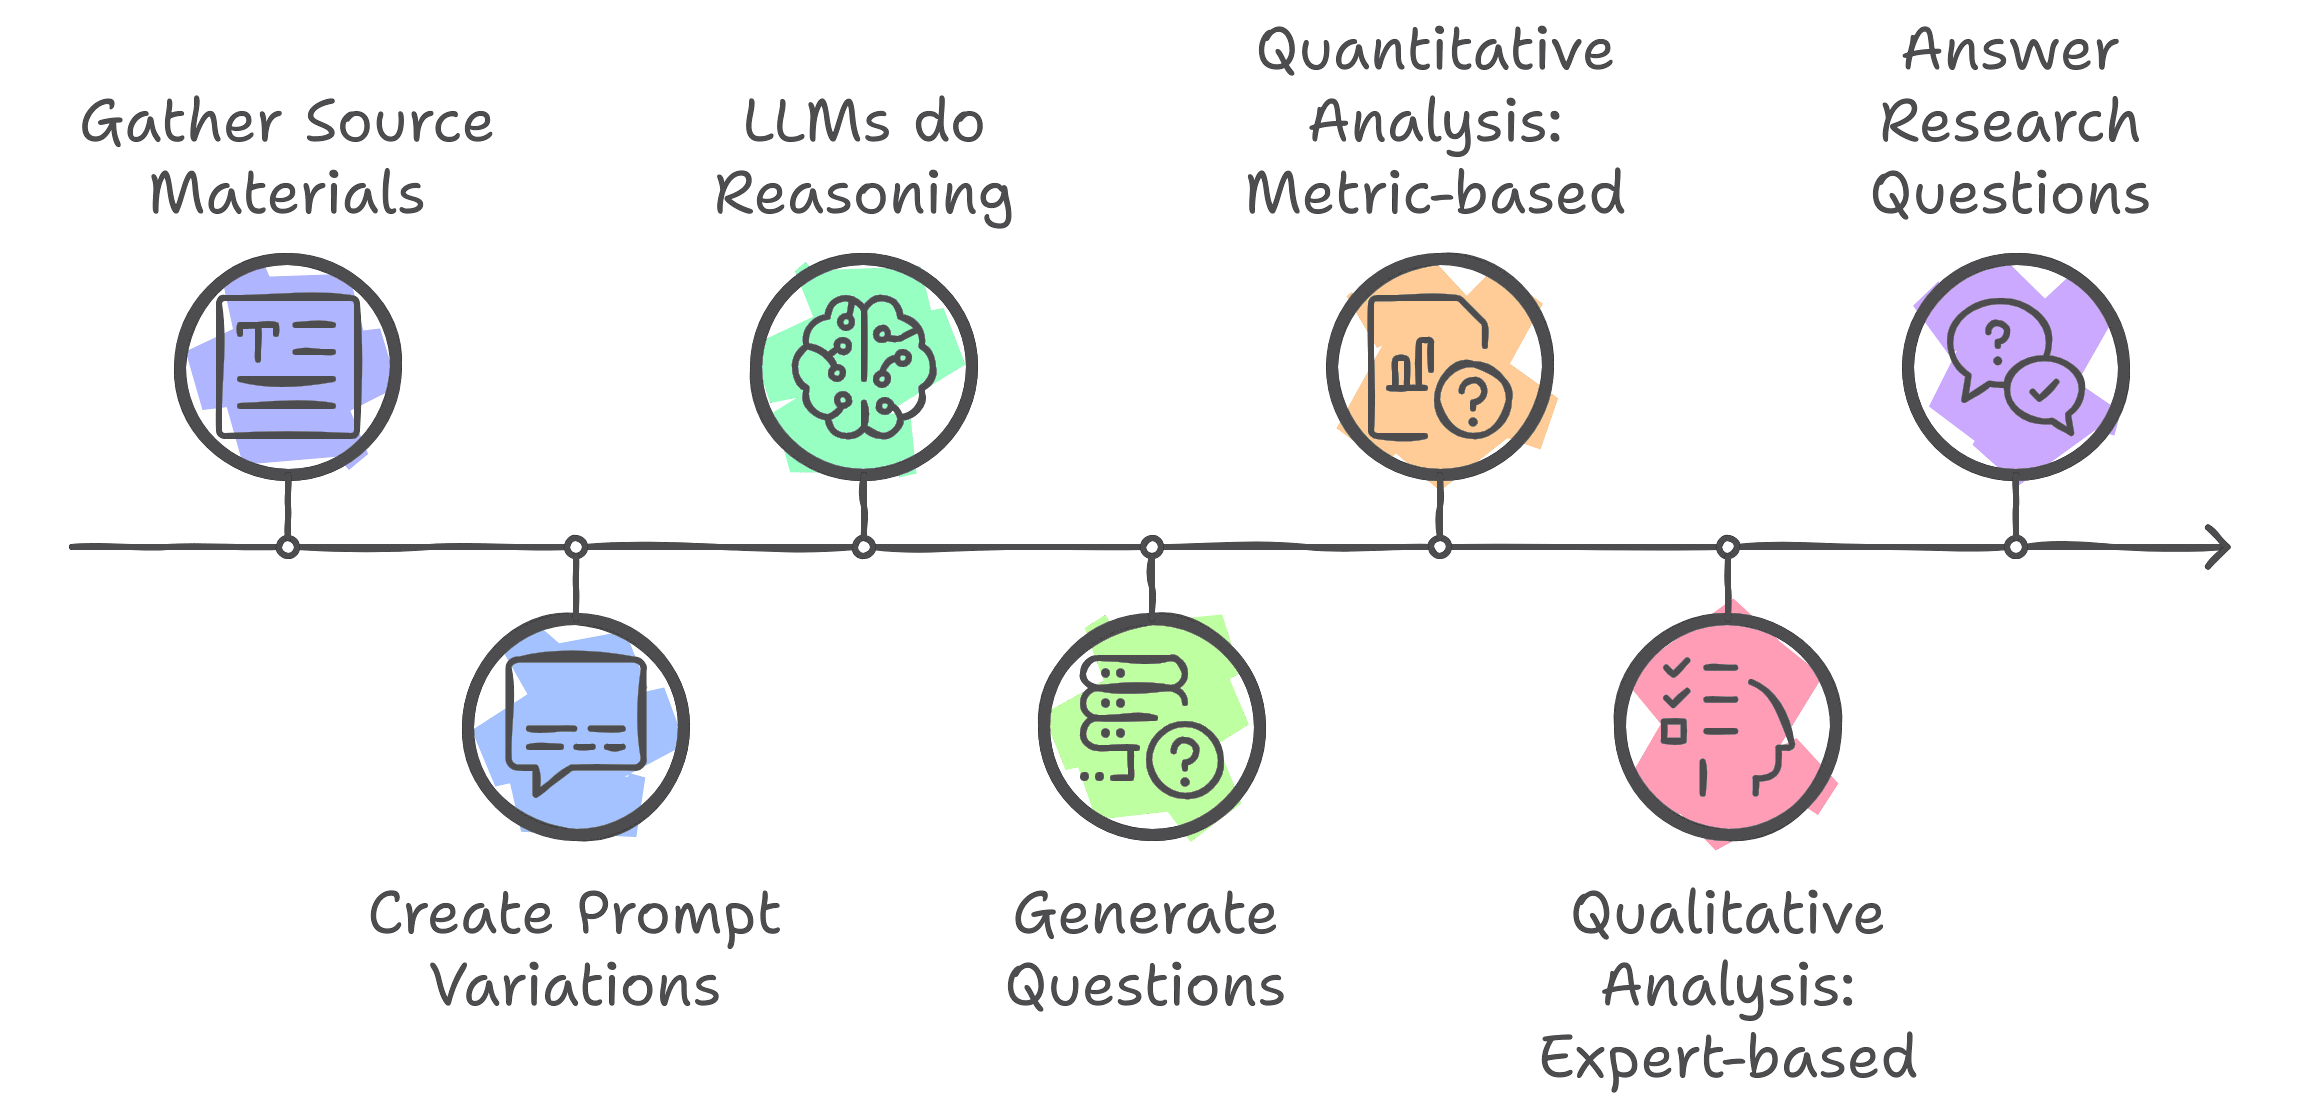
\includegraphics[width=.9\textwidth]{../10_extra/approach.png}
    \caption[Experimental Pipeline.]{Experimental Pipeline\footnotemark.}
    \label{fig:experiment-overview}
\end{figure}
\footnotetext{created with \url{https://www.napkin.ai/}, accessed 05/24/2025}
\vspace{-1em}
    
\subsection{Selection of Resources}
\label{sec:selection-resources}

To ensure the experiments were well-structured and relevant, a variety of resources were selected. This covers the source materials and the \ac{llms} used in the experiments for \ac{aqg}.

\object{Selection of Source Materials}
Focusing on the ISO-OSI model, the following materials, illustrated in its \bfhyperref{sec:source_materials}{Appendices} subsection, were diversely used to generate the experiments' questions:

\begin{itemize}
    \item \bfhyperref{sec:script-common}{Lecture Slides} \textbf{(extracted Parts)}: Dealing with reference architectures, the ISO-OSI model is presented in detail by the primary thesis supervisor. The lecture slides are in German and were used for \ac{aqg} for both experiments.
    \item \bfhyperref{sec:transcript}{Transcript} \textbf{(Lecture's Video Parts)}: The transcript of the extracted slides is in German and was also used to generate questions for the first experiment.
    \item \bfhyperref{sec:tanenbaum}{Book's Excerpt} \textbf{(from \enquote{Computer Networks})} \cite{tanenbaum_computer_2013}: This book is in English and was used to generate questions for both experiments, with a detailed description of the ISO-OSI model, including all seven layers.
\end{itemize}

\pagebreak

To properly challenge the \ac{llms} in their multilingual capabilities, each source material was kept in its original language: German for the lecture slides and its transcript, the book excerpt in English.

% \pagebreak

\object{Selection of \ac{llms}} A total of four \ac{llms} were selected for both experiments, which belong to the current state-of-the-art in the field of \ac{llms} and are publicly available to certain degrees, and incorporate reasoning capabilities. The selected models are:
Anthropic Claude 3.7 Sonnet \cite{anthropic_claude_2025},
    DeepSeek R1 \cite{deepseek-ai_deepseek-r1_2025},
    Google Gemini 2.5 Flash \cite{kavukcuoglu_gemini_2025}, and
    OpenAI o3 \cite{openai_openai_2025-1}.

\vspace{1em}

o3 and Claude 3.7 Sonnet were accessed through their Python APIs\footnote{\label{fn:openai-api}\url{https://github.com/openai/openai-python}, accessed 05/09/2025}\footnote{\label{fn:anthropic-api}\url{https://github.com/anthropics/anthropic-sdk-python}, accessed 05/09/2025}, incurring costs per usage. This access method was necessary as the chosen models were not available to the required extent through other means. In contrast, Gemini 2.5 Flash was utilized via Google's Python API\footnote{\label{fn:google-api}\url{https://github.com/googleapis/python-genai}, accessed 05/09/2025}, which offers a free usage tier. To manage costs while maintaining a robust set of \ac{llms}, DeepSeek R1, a comparatively less expensive yet highly capable \ac{llm}, was accessed free of charge via its website\footnote{\label{fn:deepseek}\url{https://chat.deepseek.com/}, accessed 05/09/2025}.

\subsection{Methodological Approach}
\label{sec:methodological-approach}

The method employed for the two experiments is outlined here. It details the specific procedures for generating questions, including the variations in source materials, \ac{llm} prompting strategies, and the targeted number of questions for each experimental condition.

\object{Experiment 1a: Content Fidelity} For the first experiment, questions were generated using the three selected source materials to compare the questions' quality. All four state-of-the-art \ac{llms} were employed. Each model was prompted using both a simple and a complex prompt. To prevent context spillover and ensure focused questioning, one question was generated per prompt for each of the seven layers of the ISO-OSI model, with the context for each layer being introduced in each distinct run. This methodology resulted in a total of
 \begin{align}4 \text{ \ac{llms}} \times 3 \text{ input sources} \times 7 \text{ layers} \times 1 \sfrac{\text{ question}}{\text{prompt}} \times 2 \text{ prompts} = 168 \text{ questions.}\end{align}

\object{Experiment 1b: Error Handling} A subsequent run focused on error handling. The four \ac{llms} were again utilized with the same prompts. For this experiment, a single input source, specifically the lecture script -- chosen for its concise and precise contextual information -- was used. Each of the seven layers of the ISO-OSI model within this source material was intentionally manipulated to introduce errors, as to be seen in its \bfhyperref{sec:script-manipulated}{Appendices} subsection. Seven questions were generated per prompt, one for each manipulated layer and run. This resulted in a total of \begin{align}4 \text{ \ac{llms}} \times 1 \text{ input source} \times 7 \text{ layers} \times 1 \sfrac{\text{ question}}{\text{prompt}} \times 2 \text{ prompts} = 56 \text{ questions.}\end{align}

\pagebreak

\object{Experiment 2: Question Formats and Bloom's Taxonomy} The second experiment focused on the generation of varied question formats and their alignment with Bloom's revised Taxonomy. Contextual information for this experiment was derived from all ISO-OSI model layers together, utilizing the precise lecture \bfhyperref{sec:script-common}{Script} by the primary thesis supervisor. The four selected \ac{llms} were employed in three distinct runs, each designed to explore different prompting parameters related to question type and cognitive complexity:

\begin{enumerate}
    \item \textit{Question Type Specification}: Prompts specified only the desired question types (Multiple-Choice and Open-Ended). For the chosen layer, each \ac{llm} was tasked six times to generate a question without mentioning a certain Bloom level for each of the two question types, resulting in \begin{align}4 \text{ \ac{llms}} \times 2 \text{ question types} \times 1 \sfrac{\text{ question}}{\text{run}}\times 6 \text{ runs} = 48 \text{ questions.}\end{align}
    \item \textit{Cognitive Level Specification}: Prompts specified only the target cognitive levels according to Bloom's Taxonomy. For the chosen layer, each \ac{llm} generated one question for six runs to get a question for each of the Bloom levels. In total, these are  \begin{align}4 \text{ \ac{llms}} \times 1 \sfrac{\text{ question}}{\text{level}} \times 6 \text{ Bloom levels} = 24 \text{ questions.}\end{align}
    \item \textit{Combined Specification}: Prompts specified both the question types (Multiple-Choice and Open-Ended) and the cognitive levels. Similar to the first run, this resulted in \begin{align}4 \text{ \ac{llms}} \times 2 \text{ question types} \times 1 \sfrac{\text{ question}}{\text{level}} \times 6 \text{ Bloom levels} = 48 \text{ questions.}\end{align}
\end{enumerate}

\object{Data Collection} The data was primarily collected using the \ac{llms} via their APIs, excepting DeepSeek being prompted on the website. The other 3 models were prompted automatically via Python to generate questions based on the given source materials. The generated questions were stored in a directory structure, particularly based on the experiment, the \ac{llm} and the source material. The question files for each prompt were stored in distinct \textit{.txt} files.

\object{Evaluation Plan} The evaluation will be conducted in two phases, one for each experiment. These employ a multi-modal assessment combining automated metrics and expert annotation -- the primary supervisor, staff members, and students -- to ensure a comprehensive quality assessment.

\begin{itemize}
    \item \textbf{Experiment 1 (Content Fidelity and Error Handling):}
    \begin{itemize}
        \item \textit{Quantitative Analysis:} In this stage, the \textit{Semantic Similarity} between each generated question and the desired source material will be evaluated. Instead of relying directly on BERTScore \cite{zhang_bertscore_2020}, the cosine similarity between the embedding vectors -- representing the source material and the generated question -- will be computed. These embeddings are obtained using a cross-lingual RoBERTa-based sentence transformer\footnote{\url{https://huggingface.co/T-Systems-onsite/cross-en-de-roberta-sentence-transformer}, accessed 05/09/2025}, which produces semantically meaningful and comparable sentence representations \cite{reimers_sentence-bert_2019}.
        
        Novel metrics such as \textit{\ac{bleurt}} and \textit{\ac{rquge}} were not employed since, on the one hand, the structure of the source material and the question differ too much, and on the other hand, gold standard answers are not available for comparison.

        Moreover, other metrics such as Perplexity are unsuitable for this task, as \enquote{the output value is based heavily on what the text and the model was trained on. This means that perplexity scores are not comparable between models or datasets}\footnote{\url{https://huggingface.co/spaces/evaluate-metric/perplexity}, accessed 06/01/2025}. Instead, to properly analyze the content adherence on a quantitative level besides the \textit{Semantic Similarity}, the \textit{Adherence Score} will be introduced in this thesis as an alternate quantitative scoring method. It will be assessed by prompting Claude 3.7 Sonnet and OpenAI o3 for every question with its desired source material to obtain acceptable results, using the mean of both \ac{llm} values. This results in a value between 0 and 1 for each question, presenting the adherence to the source material.

        \item \textit{Qualitative Analysis:} This phase involves a blind-test with expert-based evaluations of the generated questions. Five experts, including the primary thesis supervisor and four scientific staff members from the same university department of Information and Communication Services, will rate a sampled question set using the concise rubric in Table \bfref{tab:exp1_criteria}. To analyze the inter-rater agreement between the experts, Fleiss' Kappa will be calculated, which is suitable for analyses carried out by at least two raters \cite{fleiss_measuring_1971}.
        
        The thesis' analysis adopts the rubric from \cite{mi_comparative_2024} -- based on criteria by \cite{moore_assessing_2022} --, which maintains a maximum score of 50 points per question. However, instead of the \textit{Bloom's Level} criterion, the \textit{Correctness}, the \textit{Value} from the lecturer's perspective, and the \textit{Language} criteria were added to address the objectives of this experiment.
        
        Since Experiment 1b examines the adherence to manipulated input texts, the \textit{Correctness} is then replaced by \textit{Manipulation Handling}, respectively. To distinguish between the \textit{Clarity} and \textit{Language} criteria, clarity focuses on content clarity and logical comprehension, while language assesses linguistic complexity and precision of expression.

\begin{table}[htbp]
           \vspace{-5em}
           \centering
           \renewcommand{\arraystretch}{1.8}
           \caption{Experiment 1 Evaluation Criteria.}
           \label{tab:exp1_criteria}
           \begin{tabularx}{\textwidth}{|Z|A|Y|}
           \rowcolor{gray!15}
           \hline
           \textbf{Criterion} & \textbf{Description} & \textbf{Scoring} \\
           \hline
           \textbf{Relevance} & Is the question relevant to the topic of the source text? & 0-10p \\
           \hline
           \textbf{Clarity} & Is the question easy to understand \& the presentation logical and clear? & 0-10p \\
           \hline
           \textbf{Answerability} & Are students likely able to answer the question based on the provided material? & 0-10p \\
           \hline
           \textbf{Challenging} & Is the question challenging? Does it encourage students to think actively? & 0-10p \\
           \hline
           \textbf{Value} & Is the question considered professionally, didactically, or technically meaningful by the instructor? & 0-10p \\
           \hline
           \textbf{Language} & Is the language used by the system sufficiently precise and comprehensible? & 0-10p \\
           \hline
           \textbf{Correctness} & \textbf{For Experiment 1a:} Is the question factually correct \& adhering to the source text? & \vspace{-1.1em}\begin{itemize} 
                \item Correct: 10p
                \item Partially correct: 5p
                \item Otherwise: 0p
            \end{itemize} \\
           \hline
           \textbf{Manipulation Handling} & \textbf{For Experiment 1b:} Does the question adhere to the manipulated input text content? & \vspace{-1.2em}\begin{itemize} 
                \item No Adherence\,/\,Model detects Manipulation: 10p
                \item Partially adheres: 5p
                \item Otherwise: 0p
            \end{itemize} \\
           \hline
           \end{tabularx}
         \end{table}
    \end{itemize}

    \vspace{0em}

    \item \textbf{Experiment 2 (Question Formats and Bloom's Taxonomy):}
    \begin{itemize}
        \item \textit{Qualitative Analysis:} As the primary focus of this experiment lies on qualitative assessment, any quantitative evaluation is discarded. To simulate a proper blind test for this experiment, a human-based analysis will be conducted as well. Three students of the secondary thesis supervisor -- from the Institute of School Pedagogy and Educational Research -- will rate a sampled question set from the second experiment. These students will evaluate the questions using the concise rubric in Table \bfref{tab:exp2_criteria}, based on the first rubric structure. Unlike Experiment 1, the \textit{Correctness} is replaced by the \textit{Bloom's Level} criterion, as \cite{mi_comparative_2024} used this criterion before. Inter-rater agreement via Fleiss' Kappa will also be calculated for this experiment.
        
        \begin{table}[htbp]
           \vspace{-5em}
           \centering
           \renewcommand{\arraystretch}{1.8}
           \caption{Experiment 2 Evaluation Criteria.}
           \label{tab:exp2_criteria}
           \begin{tabularx}{\textwidth}{|Z|A|Y|}
           \rowcolor{gray!15}
           \hline
           \textbf{Criterion} & \textbf{Description} & \textbf{Scoring} \\
           \hline
           \textbf{Relevance} & Is the question relevant to the topic of the source text? & 0-10p \\
           \hline
           \textbf{Clarity} & Is the question easy to understand \& the presentation logical and clear? & 0-10p \\
           \hline
           \textbf{Answerability} & Are students likely able to answer the question based on their knowledge level? & 0-10p \\
           \hline
           \textbf{Challenging} & Is the question challenging? Does it encourage students to think actively? & 0-10p \\
           \hline
           \textbf{Value} & Is the question considered professionally, didactically, or technically meaningful by the instructor? & 0-10p \\
           \hline
           \textbf{Language} & Is the language used by the system sufficiently precise and comprehensible? & 0-10p \\
           \hline
           \multirow{2}{*}{\textbf{Bloom's Level}} & \textbf{When Bloom level is specified:} Does the question adhere to the given Bloom level? & \vspace{-1.1em} \begin{itemize}
                \item Correct: 10p
                \item Off by one: 5p
                \item Otherwise: 0p
            \end{itemize} \\
           \cline{2-3}
            & \textbf{When no Bloom level is specified:} Which Bloom level does the question demonstrate? & \vspace{-1.2em} \begin{itemize}
                \item Creating: 10p
                \item Evaluating: 8.5p
                \item Analyzing: 7p
                \item Applying: 4.5p
                \item Understanding: 3p
                \item Remembering: 1.5p
            \end{itemize} \\
           \hline
           \end{tabularx}
         \end{table}
    \end{itemize}
\end{itemize}

\pagebreak

Since the qualitative analyses for Experiments 1 and 2 shall be valid and as unbiased as possible, these are conducted as certain blind tests. To achieve this, the evaluators will not be aware of the used methods to generate each question. This involves the model's name, the kind of prompt used, the specified question type and the desired Bloom level for each question. Additionally, to properly analyze criteria such as \textit{Relevance}, \textit{Answerability} and \textit{Correctness}, the evaluators will be provided with the source material each question is based on. 

Furthermore, to properly score the \textit{Bloom's Level} -- based on the guideline in Table \bfref{tab:exp2_criteria}, the evaluators shall return solely the Bloom level they perceive for each question. The proper scoring then will be done automatically based on the returned Bloom level, since the raters will not be aware of the desired Bloom level for each question. This is focused because various questions of the sampling set were generated based on prompting the desired Bloom level.

Details about the Implementation and Execution for the entire experimental setup will be presented in the section \bfhyperref{sec:implementation-and-execution}{below}. The results and discussion of the evaluation will then be presented in Section \bfref{sec:evaluation}.
